\documentclass[UTF8,a4paper,zihao=-4]{ctexart}

\usepackage[left=2.35cm,right=2.35cm,top=2.45cm,bottom=2.45cm]{geometry}
\usepackage{amsmath,amssymb}
\usepackage{booktabs,longtable,tabularx,array,multirow}
\usepackage{graphicx,float,caption,subcaption}
\usepackage{xcolor}
\usepackage{listings}
\usepackage{hyperref,xurl,seqsplit}
\usepackage{fancyhdr}
\usepackage{enumitem}
\usepackage[most]{tcolorbox}
\usepackage{siunitx}
\usepackage{microtype}

\definecolor{navy}{HTML}{274C77}
\definecolor{teal}{HTML}{2A6F6B}
\definecolor{coral}{HTML}{C65D5D}
\definecolor{paper}{HTML}{F6F8FA}
\definecolor{codebg}{HTML}{F3F5F7}
\definecolor{codegreen}{HTML}{1E6B52}
\definecolor{codepurple}{HTML}{6F42C1}

\hypersetup{
  colorlinks=true,
  linkcolor=navy,
  citecolor=teal,
  urlcolor=coral,
  pdftitle={网络安全创新创业实践 7.20 作业一},
  pdfauthor={课程作业}
}
\urlstyle{same}

\pagestyle{fancy}
\fancyhf{}
\fancyhead[L]{网络安全创新创业实践}
\fancyhead[R]{7.20 作业一}
\fancyfoot[C]{\thepage}
\renewcommand{\headrulewidth}{0.4pt}
\setlength{\headheight}{15pt}

\setlength{\parindent}{2em}
\setlength{\parskip}{0.25em}
\setlist{nosep,leftmargin=2.2em}
\captionsetup{font=small,labelfont=bf}
\renewcommand{\arraystretch}{1.22}

\lstdefinestyle{pythonstyle}{
  language=Python,
  backgroundcolor=\color{codebg},
  basicstyle=\ttfamily\scriptsize,
  keywordstyle=\color{codepurple}\bfseries,
  stringstyle=\color{codegreen},
  commentstyle=\color{gray},
  numbers=left,
  numberstyle=\tiny\color{gray},
  stepnumber=1,
  numbersep=8pt,
  frame=single,
  rulecolor=\color{gray!35},
  breaklines=true,
  breakatwhitespace=false,
  showstringspaces=false,
  keepspaces=true,
  columns=fullflexible,
  tabsize=4,
  captionpos=b
}
\lstdefinestyle{datastyle}{
  backgroundcolor=\color{codebg},
  basicstyle=\ttfamily\scriptsize,
  frame=single,
  rulecolor=\color{gray!35},
  breaklines=true,
  columns=fullflexible,
  showstringspaces=false
}

\newtcolorbox{resultbox}[1][]{
  enhanced,
  colback=teal!5,
  colframe=teal!75!black,
  boxrule=0.8pt,
  arc=1.5mm,
  title=#1,
  fonttitle=\bfseries
}
\newtcolorbox{warningbox}[1][]{
  enhanced,
  colback=coral!5,
  colframe=coral!80!black,
  boxrule=0.8pt,
  arc=1.5mm,
  title=#1,
  fonttitle=\bfseries
}

\begin{document}

\begin{titlepage}
  \centering
  \vspace*{1.8cm}
  {\zihao{1}\bfseries 网络安全创新创业实践\par}
  \vspace{0.8cm}
  {\color{navy}\rule{0.78\textwidth}{1.4pt}\par}
  \vspace{1.25cm}
  {\zihao{2}\bfseries 7月20日作业一\par}
  \vspace{0.45cm}
  {\zihao{3}\bfseries Bitcoin 测试网络交易发送、逐字节解析\par}
  {\zihao{3}\bfseries 与完整区块验证\par}
  \vspace{1.8cm}
  \begin{tcolorbox}[width=0.76\textwidth,colback=paper,colframe=navy!65,arc=1mm]
    \centering
    \begin{tabular}{rl}
      姓名：& \rule{7cm}{0.4pt}\\[0.7em]
      学号：& \rule{7cm}{0.4pt}\\[0.7em]
      班级：& \rule{7cm}{0.4pt}\\[0.7em]
      完成日期：& 2026年7月20日
    \end{tabular}
  \end{tcolorbox}
  \vfill
  {\large 课程实验报告\par}
  \vspace{0.8cm}
\end{titlepage}

\pagenumbering{Roman}
\begin{abstract}
本作业面向 Bitcoin 测试网络，完成了两笔真实 Testnet4 交易的构造与广播，并从线协议字节出发独立实现交易、区块和 Script 的解析与验证。第一笔交易花费 5 个锁定为 \texttt{P2WSH(SHA256(OP\_TRUE))} 的公开教学输出，将 \num{1650} sat 合并为课程钱包的 \num{1000} sat 输出；第二笔交易由课程专用私钥按 BIP143 构造签名原像，使用 RFC6979 确定性 nonce 和 low-S ECDSA 签名，将 \num{400} sat 发往接收地址，并产生 \num{318} sat 找零。两个广播交易的 txid 分别为 \texttt{4aa330ae...25f7a} 和 \texttt{ad00f80a...9ac105}。

实现未调用第三方 Bitcoin 解析库，而是使用 Python 标准库完成 CompactSize、大小端转换、SegWit 序列化、txid/wtxid、Merkle 树、紧凑难度目标、secp256k1 点运算、DER 签名和 P2WPKH/P2WSH Script 审计。课程签名交易的 \num{223} 个字节以及包含父交易的已确认完整区块的 \num{4045} 个字节均被逐字节映射到唯一协议字段；ECDSA、CleanStack、Merkle 根和 PoW 独立重算全部通过。父交易已在高度 \num{144878} 确认，子交易在最终采样时仍为 mempool 未确认状态。另以一笔已确认默认 Signet P2WPKH 交易和其 \num{74123} 字节区块作为回归样本。报告给出题目原文、理论、完整计算、运行结果、图形证据、测试和全部源代码。

\noindent\textbf{关键词：}Bitcoin；Testnet4；SegWit；P2WPKH；P2WSH；BIP143；ECDSA；Merkle 树；逐字节解析
\end{abstract}

\tableofcontents
\clearpage
\pagenumbering{arabic}

\section{作业原文、目标与完成边界}

\subsection{原始 Project 要求}

课程截图中的 Project 原文为：

\begin{quote}
\textbf{Project: send a tx on Bitcoin testnet, and parse the tx data down to every bit \&\& parse a whole block, try to calc each byte with script.}
\end{quote}

结合课件同页的 Blockchain、Block、Tx/Coinbase tx、Input、Output、Locking Script、Unlocking Script 与 PoW 上下文，本报告将要求严格化为以下可验收目标：

\begin{enumerate}
  \item 在公开 Bitcoin 测试网络广播至少一笔由本实验构造的交易，并保留 raw transaction、txid、节点返回和时间证据；
  \item 不依赖浏览器的解码结果，从原始字节解析交易，给每个字节标注十六进制、8 位二进制和所属字段；
  \item 从 80 字节区块头到最后一笔交易完整解析一个区块，重算区块哈希、目标值、PoW 与 Merkle 根，并证明无遗漏或重叠字节；
  \item 对锁定/解锁条件逐步执行 Script，至少覆盖本实验的 P2WSH \texttt{OP\_TRUE} 与 P2WPKH ECDSA 两条路径；
  \item 附代码、运行结果、截图/可视化、自动化测试与引用资料。
\end{enumerate}

\begin{figure}[H]
  \centering
  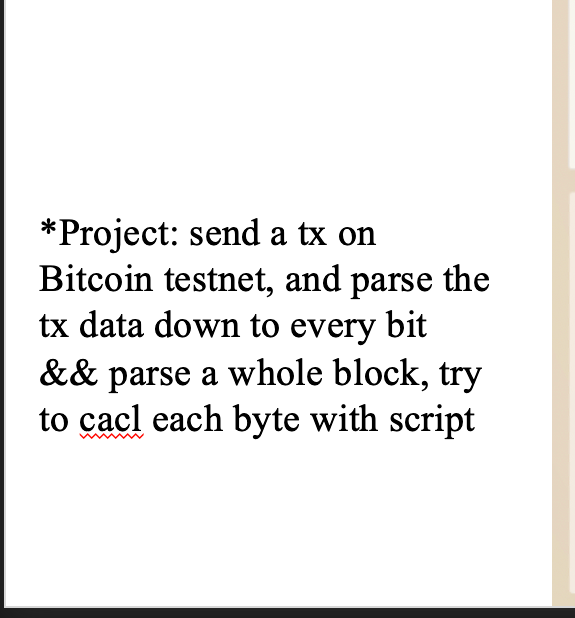
\includegraphics[width=0.58\textwidth]{figures/assignment1_project_crop.png}
  \caption{课程截图中作业一的 Project 原文（裁剪自原始图片）}
  \label{fig:assignment-original}
\end{figure}

\subsection{网络选择与诚实性说明}

实验选择 \textbf{Bitcoin Testnet4}。BIP94 将 Testnet4 定义为替代 Testnet3 的新测试网络，并说明它除少量测试网难度规则外与主网共用共识规则，且从创世块起启用截至 2024 年 5 月主网已有软分叉\cite{bip94}。因此它比长期运行且存在 block storm 问题的 Testnet3 更适合作为本课程实验环境。

本实验先后尝试默认 Signet 水龙头；服务端接受排队请求但未产生 UTXO。为避免把离线交易冒充广播交易，最终采用 Testnet4 上\emph{锁定脚本明确授权任何人花费}的 \texttt{P2WSH}\allowbreak\texttt{(OP\_TRUE)} 教学输出作为启动资金。该行为不使用、猜测或泄露任何第三方私钥：授权完全来自链上 Script。随后课程钱包使用自己的 ECDSA 私钥花费收到的输出。报告只将节点明确返回 txid 的交易称为“已广播”；在采样时尚未入块的交易标注为“mempool 已接受、未确认”。

\section{规范与数学基础}

\subsection{UTXO 与交易序列化}

Bitcoin 交易不直接修改账户余额，而是引用既有未花费交易输出（UTXO），并创建新输出。输入通过
\[
  \text{outpoint}=\text{prev\_txid}_{32\,\mathrm{B}}\,\|\,\text{vout}_{4\,\mathrm{B}}
\]
定位被花费输出。金额为 8 字节小端无符号整数，单位 satoshi。输入数、输出数、脚本长度和 witness 项数使用 CompactSize：小于 \texttt{0xfd} 时占 1 字节，否则由前缀 \texttt{fd}/\texttt{fe}/\texttt{ff} 指示 2/4/8 字节小端载荷。实现额外拒绝非最短编码，避免同值多编码造成歧义。

BIP141 对含 witness 的交易定义\cite{bip141}：
\[
\begin{aligned}
\text{wire}={}&[\text{version}][00][01][\text{vin}][\text{vout}]\\
               & [\text{witness per input}][\text{locktime}].
\end{aligned}
\]
其中 txid 仍为传统（不含 marker、flag、witness）序列化的双 SHA-256，而 wtxid 为完整 witness 序列化的双 SHA-256；哈希在常见显示形式中反转字节序：
\[
\mathrm{txid}=\operatorname{rev}(\mathrm{SHA256d}(\mathrm{ser}_{\rm stripped}(tx))),\quad
\mathrm{wtxid}=\operatorname{rev}(\mathrm{SHA256d}(\mathrm{ser}_{\rm witness}(tx))).
\]
交易权重和虚拟大小为
\[
W=4S_{\rm stripped}+(S_{\rm total}-S_{\rm stripped}),\qquad
vsize=\left\lceil\frac{W}{4}\right\rceil .
\]

\subsection{Bech32 与 witness program}

BIP173 规定测试网 SegWit 地址的人类可读前缀为 \texttt{tb}，数据部分先把 witness program 从 8 位组转换为 5 位组，再附加 BCH 类校验码\cite{bip173}。本实验使用 witness v0：

\begin{itemize}
  \item P2WPKH：\texttt{00 14 <HASH160(pubkey)>}，program 长度 20 字节；
  \item P2WSH：\texttt{00 20 <SHA256(witnessScript)>}，program 长度 32 字节。
\end{itemize}

\subsection{P2WSH(OP\_TRUE) 的公开授权}

本实验启动资金的 witnessScript 仅为 \texttt{51}，即 \texttt{OP\_TRUE}。其 SHA-256 为
\[
\seqsplit{4ae81572f06e1b88fd5ced7a1a000945432e83e1551e6f721ee9c00b8cc33260}.
\]
因此锁定脚本是
\[
\texttt{00204ae81572f06e1b88fd5ced7a1a000945432e83e1551e6f721ee9c00b8cc33260}.
\]
BIP141 要求 P2WSH 的 witness 最后一项的 SHA-256 等于 32 字节 program，然后执行该 witnessScript，最终栈必须恰有一个 TRUE\cite{bip141}。本例 witness 为 \texttt{[51]}，哈希相等后执行 \texttt{OP\_TRUE}，最终栈为 \texttt{[01]}。这就是链上显式的“任何人可花费”授权。

\subsection{BIP143 签名原像}

P2WPKH 的实际 scriptCode 为传统 P2PKH 模板
\[
\texttt{76 a9 14 <20-byte-pubkey-hash> 88 ac},
\]
即 \texttt{OP\_DUP OP\_HASH160 PUSH20 OP\_EQUALVERIFY OP\_CHECKSIG}。对 \texttt{SIGHASH\_ALL}，BIP143 的原像为\cite{bip143}：
\[
\begin{aligned}
&nVersion\|hashPrevouts\|hashSequence\|outpoint\|scriptCode\\
&\quad\|amount\|nSequence\|hashOutputs\|nLockTime\|sighashType.
\end{aligned}
\]
其中三个聚合哈希均为双 SHA-256。与旧算法相比，BIP143 将被花费输出的金额纳入承诺，并通过聚合哈希避免多输入交易签名验证的二次复杂度。

\subsection{secp256k1 ECDSA}

曲线和基点阶为
\[
E:\ y^2=x^3+7\pmod p,
\]
\[
p=2^{256}-2^{32}-977.
\]
\begin{center}
\small
$n={}$\texttt{\seqsplit{FFFFFFFFFFFFFFFFFFFFFFFFFFFFFFFEBAAEDCE6AF48A03BBFD25E8CD0364141}}.
\end{center}
私钥为 $d\in[1,n-1]$，公钥 $Q=dG$。对摘要整数 $z$，选择 nonce $k$，令
\[
R=kG=(x_R,y_R),\quad r=x_R\bmod n,\quad s=k^{-1}(z+rd)\bmod n.
\]
验证时计算
\[
w=s^{-1},\quad X=(zw)G+(rw)Q,
\]
接受条件为 $X\neq\mathcal O$ 且 $x_X\bmod n=r$。实现采用 RFC6979 HMAC-SHA256 确定性 nonce，并令 $s\leftarrow\min(s,n-s)$ 满足 Bitcoin 的 low-S 规范，从而移除 ECDSA 的 $s\leftrightarrow n-s$ 可塑性。

\subsection{区块头、目标值与 Merkle 根}

区块原始数据由 80 字节头、交易数 CompactSize 和连续交易组成。头字段依次为 version、previous block hash、Merkle root、time、nBits、nonce。区块标识为
\[
\mathrm{blockhash}=\operatorname{rev}(\mathrm{SHA256d}(header)).
\]
若 \texttt{nBits} 的最高字节为指数 $e$，低 23 位为系数 $c$，目标值为
\[
T=c\cdot 256^{e-3},\qquad \operatorname{int}(\mathrm{SHA256d}(header))\le T.
\]
Merkle 树叶子为 txid 的内部字节序；每层两两连接后双 SHA-256，奇数节点复制末项，直到得到根。程序把重算根与区块头中的 32 字节字段比较。

\section{设计与实现}

\subsection{工程结构}

代码位于作业根目录的 \path{code/} 子目录，职责见表~\ref{tab:files}。

\begin{table}[H]
\centering
\caption{作业一代码与产物结构}
\label{tab:files}
\begin{tabularx}{\textwidth}{>{\ttfamily\small}p{0.35\textwidth} >{\raggedright\arraybackslash}X}
\toprule
文件 & 职责\\
\midrule
code/bitcoin\_codec.py & secp256k1、RFC6979/low-S ECDSA、DER、Bech32、CompactSize、交易/区块解析、BIP143、P2WPKH/P2WSH Script\\
code/wallet\_tool.py & 测试网钱包生成、UTXO 查询、1 入 2 出 P2WPKH 构造、签名、广播与证据 JSON\\
code/claim\_op\_true\_utxos.py & 按链上公开条件花费 P2WSH(OP\_TRUE) 输出，构造并广播启动交易\\
code/chain\_analyzer.py & 拉取 raw tx/raw block，逐字段反序列化，输出每字节 8 位映射、CSV/JSON，并独立验证\\
code/visualize\_results.py & 从 JSON/CSV 生成字节布局、Script 栈和运行汇总图\\
code/test\_bitcoin\_codec.py & 6 项确定性回归测试\\
output/ & raw hex、逐字节映射、字段表、区块交易索引、Script trace、广播证据和图片\\
\bottomrule
\end{tabularx}
\end{table}

\subsection{防错约束}

解析器不是“尽可能读”而是“精确消费”：任何越界、非最短 CompactSize、字段重叠、尾随字节或重序列化不一致都会抛出异常。对长度为 $L$ 的 raw data，字节标注器建立 $L$ 个初始为 \texttt{UNCLAIMED} 的槽位；每个 Span 只能覆盖未占用槽位，完成后必须不存在 \texttt{UNCLAIMED}。因此
\[
\sum_i (end_i-start_i)=L
\]
只是必要条件，程序还同时验证 Span 互不重叠，避免“重复计算恰好掩盖遗漏”。

网络层优先调用系统 \texttt{curl} 并设置超时与重试，保留 \texttt{urllib} 回退；密码学与协议解析不依赖网络库或第三方 Bitcoin SDK。

\section{真实交易构造与广播}

\subsection{课程地址}

课程专用 Testnet4 地址如下，报告不披露私钥：

\begin{itemize}
  \item 发送/找零地址：\texttt{tb1qw0mgkymm78hd270asxdcvhlucfhjw72t4ajxge}；
  \item 接收地址：\texttt{tb1qkts77kng6xv0rxldrjjfctk5jmf5nx3ltsndlw}。
\end{itemize}

私钥文件仅标注为测试网络密钥，并明确禁止发送主网 BTC。父交易和子交易均由程序先本地重算 txid，再 POST raw hex 到 Esplora 兼容的 Testnet4 \texttt{/api/tx}；仅当服务器返回值与本地 txid 完全相同才写入 \texttt{broadcast\_txid}。

\subsection{父交易：P2WSH(OP\_TRUE) 合并}

父交易于北京时间 2026-07-20 15:31:26 广播。核心结果见表~\ref{tab:parent}。

\begin{table}[H]
\centering
\caption{父交易广播结果}
\label{tab:parent}
\begin{tabularx}{\textwidth}{p{0.28\textwidth} X}
\toprule
项目 & 值\\
\midrule
txid & \ttfamily\seqsplit{4aa330ae4ecf52c82f38d22149b2b7da79f928e1cdad47bb33b553c093a25f7a}\\
wtxid & \ttfamily\seqsplit{7ea8089a0b477ef55a2d1ae80bd24f2025ef6020b1207e224177e9ff52f8b9b7}\\
输入/输出 & 5 个 $330$ sat P2WSH(OP\_TRUE) 输入；1 个 $1000$ sat P2WPKH 输出\\
金额守恒 & $5\times330=1650=1000+650$ sat\\
大小 & total=263 B，stripped=246 B，weight=1001 WU，vsize=251 vB\\
手续费率 & $650/251\approx2.590$ sat/vB\\
链上状态 & 节点返回值与本地 txid 一致；已在高度 144878 确认\\
浏览器 & \url{https://mempool.space/testnet4/tx/4aa330ae4ecf52c82f38d22149b2b7da79f928e1cdad47bb33b553c093a25f7a}\\
\bottomrule
\end{tabularx}
\end{table}

对 5 个输入逐一得到
\[
\mathrm{SHA256}(\texttt{51})=
\seqsplit{4ae81572f06e1b88fd5ced7a1a000945432e83e1551e6f721ee9c00b8cc33260},
\]
与各 prevout 的 witness program 完全相同；执行 \texttt{OP\_TRUE} 后最终栈均为 \texttt{[01]}，5/5 输入通过 CleanStack。

\subsection{子交易：课程私钥 P2WPKH 签名}

子交易于北京时间 2026-07-20 15:32:13 广播。它花费父交易的 1000 sat 输出，将 400 sat 发到接收地址，318 sat 找零，支付 282 sat 手续费。结果见表~\ref{tab:child}。

\begin{table}[H]
\centering
\caption{课程私钥签名交易结果}
\label{tab:child}
\begin{tabularx}{\textwidth}{p{0.28\textwidth} X}
\toprule
项目 & 值\\
\midrule
txid & \ttfamily\seqsplit{ad00f80a9c85264ebf3ca4299d61cca06efba0487223d4e6caa9d9e58e9ac105}\\
wtxid & \ttfamily\seqsplit{56508ced1dc61e19699ce54b23728fbf076b95bb737ead63074926bde6661825}\\
输入 & 父交易 \texttt{4aa330ae...25f7a:0}，1000 sat\\
输出 0 & 400 sat，\ttfamily\small\seqsplit{0014b2e1ef5a68d198f19bed1ca49c2ed496d3499a3f}\\
输出 1 & 318 sat，\ttfamily\small\seqsplit{001473f68b137bf1eed579fd819b865ffcc26f27794b}\\
金额守恒 & $1000=400+318+282$ sat\\
大小 & total=223 B，stripped=113 B，weight=562 WU，vsize=141 vB\\
手续费率 & $282/141=2.000$ sat/vB\\
链上状态 & 节点返回值与本地 txid 一致；最终采样时仍在 mempool，未确认\\
浏览器 & \url{https://mempool.space/testnet4/tx/ad00f80a9c85264ebf3ca4299d61cca06efba0487223d4e6caa9d9e58e9ac105}\\
\bottomrule
\end{tabularx}
\end{table}

完整 raw transaction 如下；为适配版心按 64 个十六进制字符换行，逐行连续拼接即为广播的原始字节流：

\begin{lstlisting}[style=datastyle]
020000000001017a5fa293c053b533bb47adcde128f979dab7b24921d2382fc852
cf4eae30a34a0000000000fdffffff029001000000000000160014b2e1ef5a68
d198f19bed1ca49c2ed496d3499a3f3e0100000000000016001473f68b137bf1
eed579fd819b865ffcc26f27794b02483045022100b62d9b08f0c3ad4047342a
89926efc9555b41f011ef38825b3f16e1edaca5faf0220522e664de587467051
5a5f6049d92d7db9875d5c05b8deda8a65007539187d6a0121027bcb30196c0f
faee495d2c054e1bf7483bfa470c08dee12cef47d729d5cb50b200000000
\end{lstlisting}

\begin{figure}[H]
  \centering
  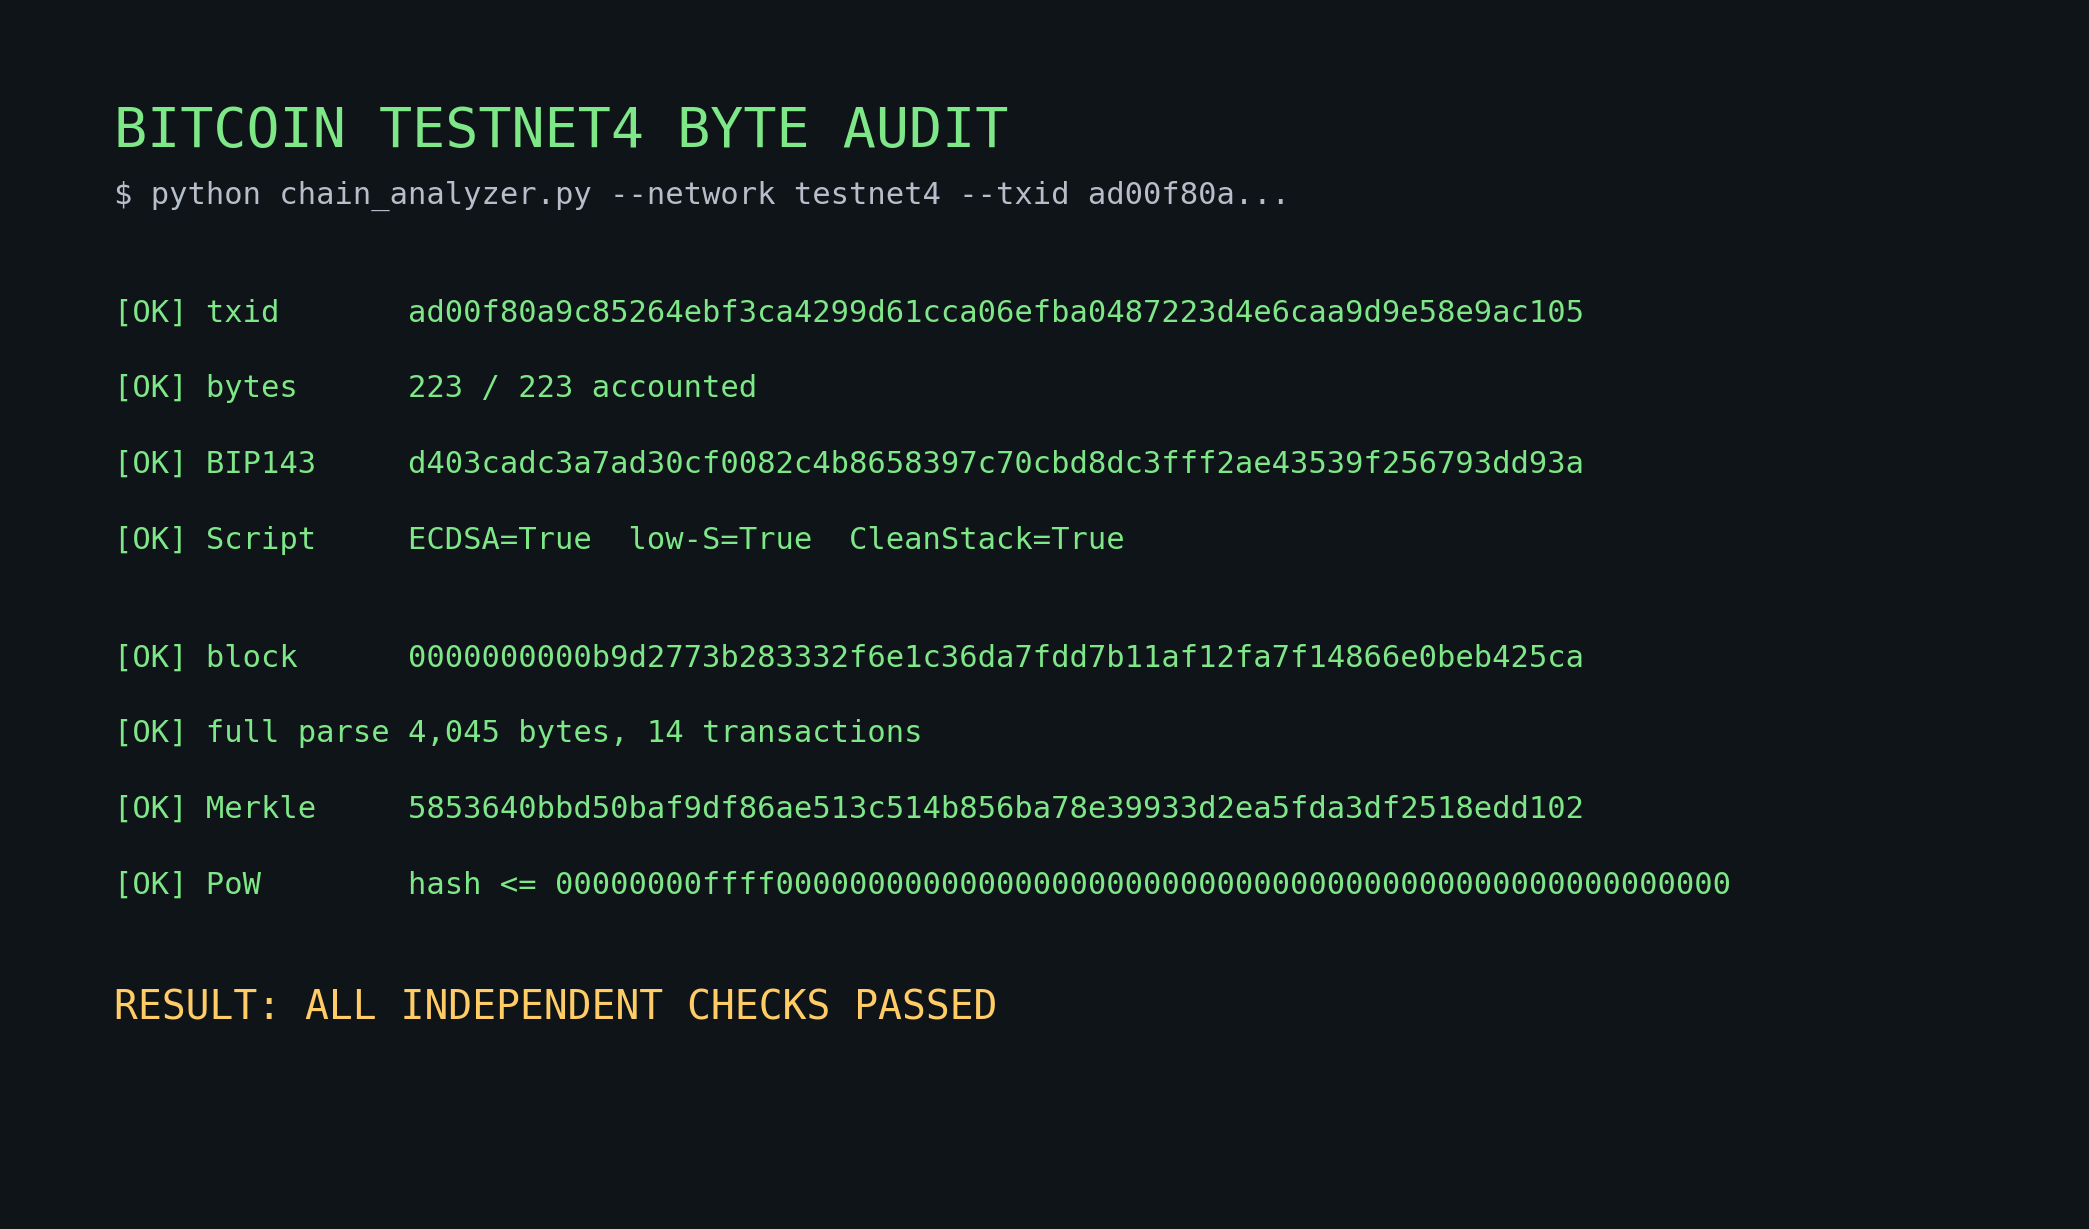
\includegraphics[width=\textwidth]{../output/figures/runtime_validation.png}
  \caption{程序根据实际 JSON 输出生成的运行验证汇总图}
  \label{fig:runtime}
\end{figure}

\section{课程签名交易逐字节解析}

\subsection{字段级完整表}

表~\ref{tab:tx-fields} 从偏移 0 连续覆盖到偏移 223；零长度 scriptSig 合法地占据区间 $[44,44)$，不消耗字节。prev txid 的 wire bytes 为小端，常见显示值需反转。

\begin{longtable}{r r r p{0.29\textwidth} p{0.39\textwidth}}
\caption{223 字节课程签名交易的字段映射}\label{tab:tx-fields}\\
\toprule
起点 & 终点 & 长度 & 字段 & wire hex / 解释\\
\midrule
\endfirsthead
\toprule
起点 & 终点 & 长度 & 字段 & wire hex / 解释\\
\midrule
\endhead
0&4&4&\texttt{version}&\texttt{02000000}，小端整数 2\\
4&5&1&\texttt{marker}&\texttt{00}，SegWit marker\\
5&6&1&\texttt{flag}&\texttt{01}，witness present\\
6&7&1&\texttt{input\_count}&\texttt{01}，1 个输入\\
7&39&32&\texttt{prev\_txid\_le}&\ttfamily\seqsplit{7a5fa293c053b533bb47adcde128f979dab7b24921d2382fc852cf4eae30a34a}\\
39&43&4&\texttt{prev\_vout}&\texttt{00000000}，索引 0\\
43&44&1&\texttt{scriptSig length}&\texttt{00}\\
44&44&0&\texttt{scriptSig}&空（native witness 必须为空）\\
44&48&4&\texttt{sequence}&\texttt{fdffffff}，$4294967293$，启用 RBF\\
48&49&1&\texttt{output\_count}&\texttt{02}\\
49&57&8&\texttt{vout[0].value}&\texttt{9001000000000000}，400 sat\\
57&58&1&\texttt{vout[0].script length}&\texttt{16}，22 B\\
58&80&22&\texttt{vout[0].scriptPubKey}&\ttfamily\seqsplit{0014b2e1ef5a68d198f19bed1ca49c2ed496d3499a3f}\\
80&88&8&\texttt{vout[1].value}&\texttt{3e01000000000000}，318 sat\\
88&89&1&\texttt{vout[1].script length}&\texttt{16}，22 B\\
89&111&22&\texttt{vout[1].scriptPubKey}&\ttfamily\seqsplit{001473f68b137bf1eed579fd819b865ffcc26f27794b}\\
111&112&1&\texttt{witness count}&\texttt{02}，2 项\\
112&113&1&\texttt{signature length}&\texttt{48}，72 B\\
113&185&72&\texttt{DER signature + type}&\ttfamily\seqsplit{3045022100b62d9b08f0c3ad4047342a89926efc9555b41f011ef38825b3f16e1edaca5faf0220522e664de5874670515a5f6049d92d7db9875d5c05b8deda8a65007539187d6a01}\\
185&186&1&\texttt{pubkey length}&\texttt{21}，33 B\\
186&219&33&\texttt{compressed pubkey}&\ttfamily\seqsplit{027bcb30196c0ffaee495d2c054e1bf7483bfa470c08dee12cef47d729d5cb50b2}\\
219&223&4&\texttt{locktime}&\texttt{00000000}，0\\
\bottomrule
\end{longtable}

\begin{figure}[H]
  \centering
  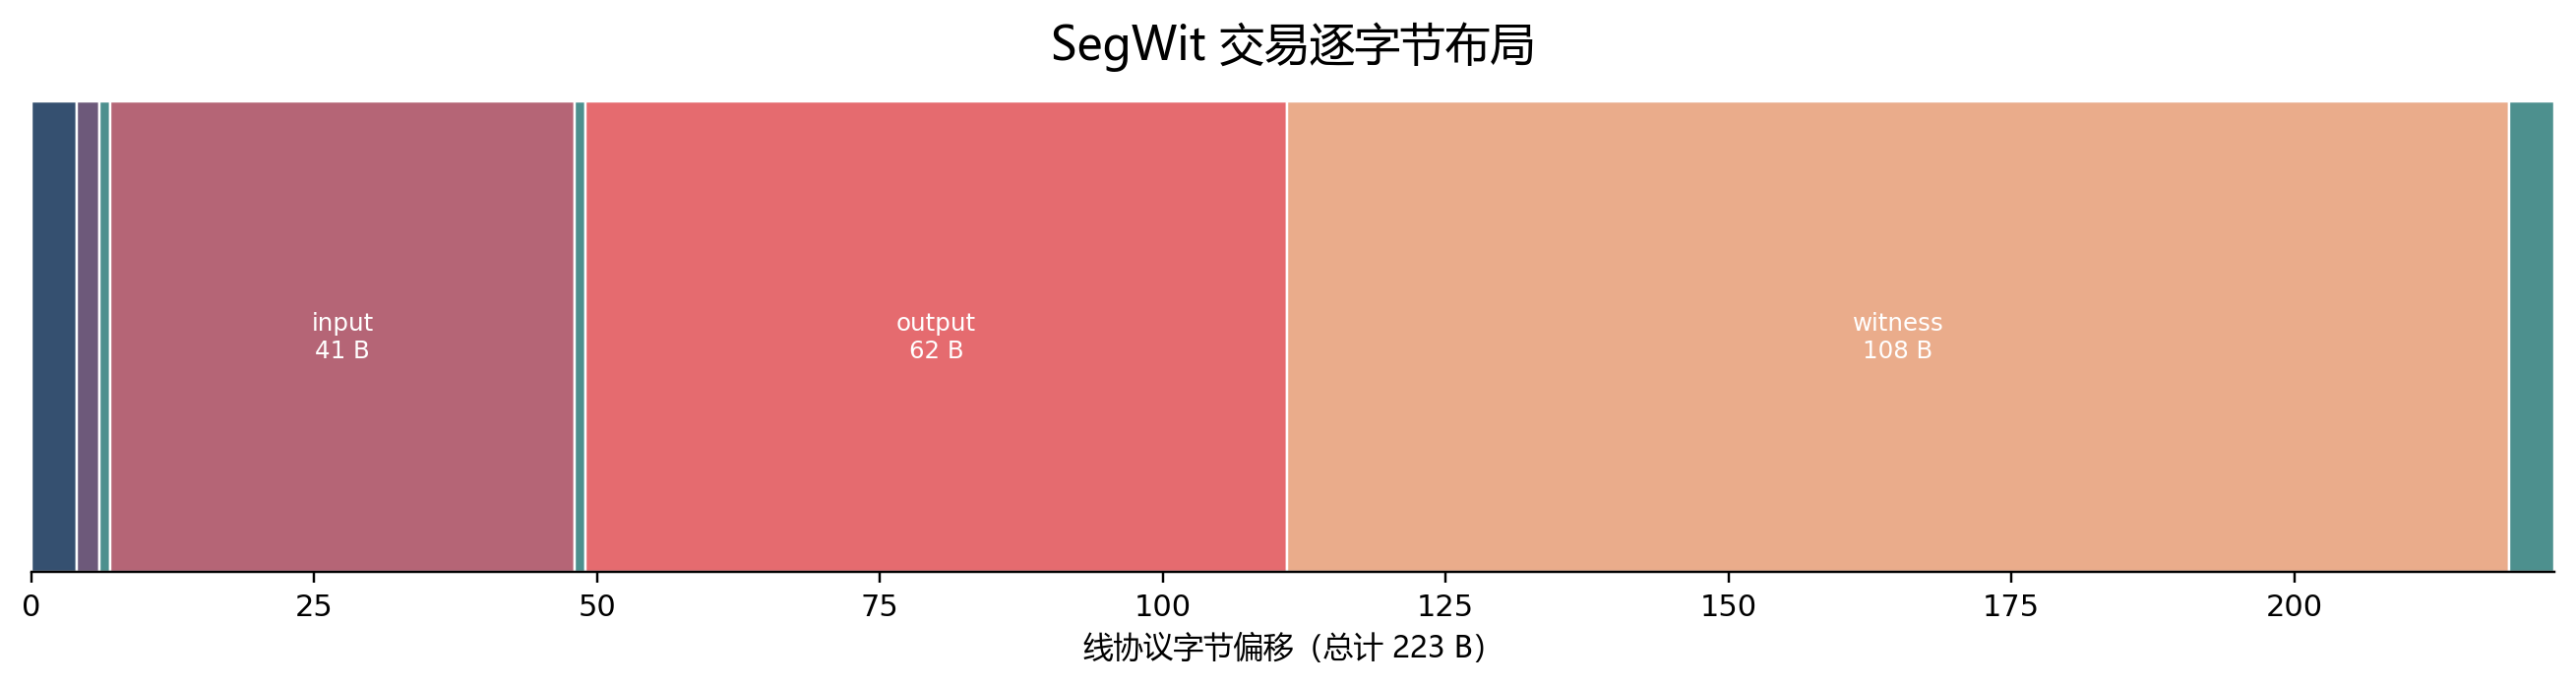
\includegraphics[width=\textwidth]{../output/figures/transaction_byte_layout.png}
  \caption{课程签名交易各字节区间的可视化}
  \label{fig:byte-layout}
\end{figure}

\subsection{位级展开示例与完整产物}

“down to every bit”按可审计形式实现为：每个 wire byte 均输出偏移、十六进制、恰好 8 位的二进制字符串和字段名。前 16 字节如下：

\begin{center}
\small
\begin{tabular}{r c c l}
\toprule
偏移 & hex & bits & 字段\\
\midrule
0&02&00000010&\texttt{tx.version}\\
1&00&00000000&\texttt{tx.version}\\
2&00&00000000&\texttt{tx.version}\\
3&00&00000000&\texttt{tx.version}\\
4&00&00000000&\texttt{tx.marker}\\
5&01&00000001&\texttt{tx.flag}\\
6&01&00000001&\texttt{tx.input\_count}\\
7&7a&01111010&\texttt{vin[0].prev\_txid\_le}\\
8&5f&01011111&\texttt{vin[0].prev\_txid\_le}\\
9&a2&10100010&\texttt{vin[0].prev\_txid\_le}\\
10&93&10010011&\texttt{vin[0].prev\_txid\_le}\\
11&c0&11000000&\texttt{vin[0].prev\_txid\_le}\\
12&53&01010011&\texttt{vin[0].prev\_txid\_le}\\
13&b5&10110101&\texttt{vin[0].prev\_txid\_le}\\
14&33&00110011&\texttt{vin[0].prev\_txid\_le}\\
15&bb&10111011&\texttt{vin[0].prev\_txid\_le}\\
\bottomrule
\end{tabular}
\end{center}

完整 223 行位图位于
\path{output/testnet4_signed_analysis/transaction_bits.txt}；完整区块 4045 行位图位于
\path{output/testnet4_signed_analysis/block_bits.txt}。这两个文件是报告电子附件，行数分别为 $223+1$ 与 $4045+1$（第一行为表头）。

\section{BIP143 与 Script 严格验证}

\subsection{签名中间值}

本输入被花费金额为 1000 sat，scriptCode 为
\[
\texttt{76a91473f68b137bf1eed579fd819b865ffcc26f27794b88ac}.
\]
程序给出的三个聚合哈希为：

\begingroup\small\ttfamily
hashPrevouts = \seqsplit{d6f3e525d7a564b2ba16490b4806fb12c5767e126f4cacda653d5db02be1d48e}\par
hashSequence = \seqsplit{caf35e5224de16efa3ccaf41070f6e7b9432b6f79551e629fca9d1c03b43bc52}\par
hashOutputs = \seqsplit{d23fabf0910579f82d571b5d5e580265b9b454353b77bb590de4e8700df80247}
\endgroup

完整原像如下；同样按 64 个十六进制字符换行，计算时不包含换行符：
\begin{lstlisting}[style=datastyle]
02000000d6f3e525d7a564b2ba16490b4806fb12c5767e126f4cacda653d5db0
2be1d48ecaf35e5224de16efa3ccaf41070f6e7b9432b6f79551e629fca9d1c
03b43bc527a5fa293c053b533bb47adcde128f979dab7b24921d2382fc852cf4e
ae30a34a000000001976a91473f68b137bf1eed579fd819b865ffcc26f27794b
88ace803000000000000fdffffffd23fabf0910579f82d571b5d5e580265b9b4
54353b77bb590de4e8700df802470000000001000000
\end{lstlisting}
故
\begin{center}
$z=\mathrm{SHA256d}(preimage)$\par
\small\ttfamily\seqsplit{d403cadc3a7ad30cf0082c4b8658397c70cbd8dc3fff2ae43539f256793dd93a}.
\end{center}
DER 解码得到
\begingroup\small\ttfamily
r = \seqsplit{b62d9b08f0c3ad4047342a89926efc9555b41f011ef38825b3f16e1edaca5faf}\par
s = \seqsplit{522e664de5874670515a5f6049d92d7db9875d5c05b8deda8a65007539187d6a}.
\endgroup
程序验证 $1\le r,s<n$、$s\le n/2$，并独立完成 $s^{-1}(zG+rQ)$ 点运算，所得横坐标模 $n$ 等于 $r$。

\subsection{P2WPKH 栈执行}

\begin{longtable}{p{0.21\textwidth}>{\raggedright\arraybackslash}p{0.47\textwidth}p{0.20\textwidth}}
\caption{课程签名输入的 Script 执行轨迹}\label{tab:script-trace}\\
\toprule
步骤 & 动作与检查 & 栈深度/结论\\
\midrule
\endfirsthead
\toprule
步骤 & 动作与检查 & 栈深度/结论\\
\midrule
\endhead
Witness 初始化 & 压入 DER 签名+\texttt{01} 与 33 B 压缩公钥 & 2\\
\texttt{OP\_DUP} & 复制栈顶公钥 & 3\\
\texttt{OP\_HASH160} & 对复制公钥计算 RIPEMD160(SHA256(pubkey)) & 3\\
\texttt{PUSH20} & 从 prevout witness program 压入 \texttt{73f68b...7794b} & 4\\
\texttt{OP\_EQUALVERIFY} & 两个 20 B 哈希相等并弹出 & 2\\
\texttt{OP\_CHECKSIG} & 用 BIP143 摘要与公钥验证 ECDSA & \texttt{[01]}\\
CleanStack & 最终恰有一个真值 & 通过\\
\bottomrule
\end{longtable}

\begin{figure}[H]
  \centering
  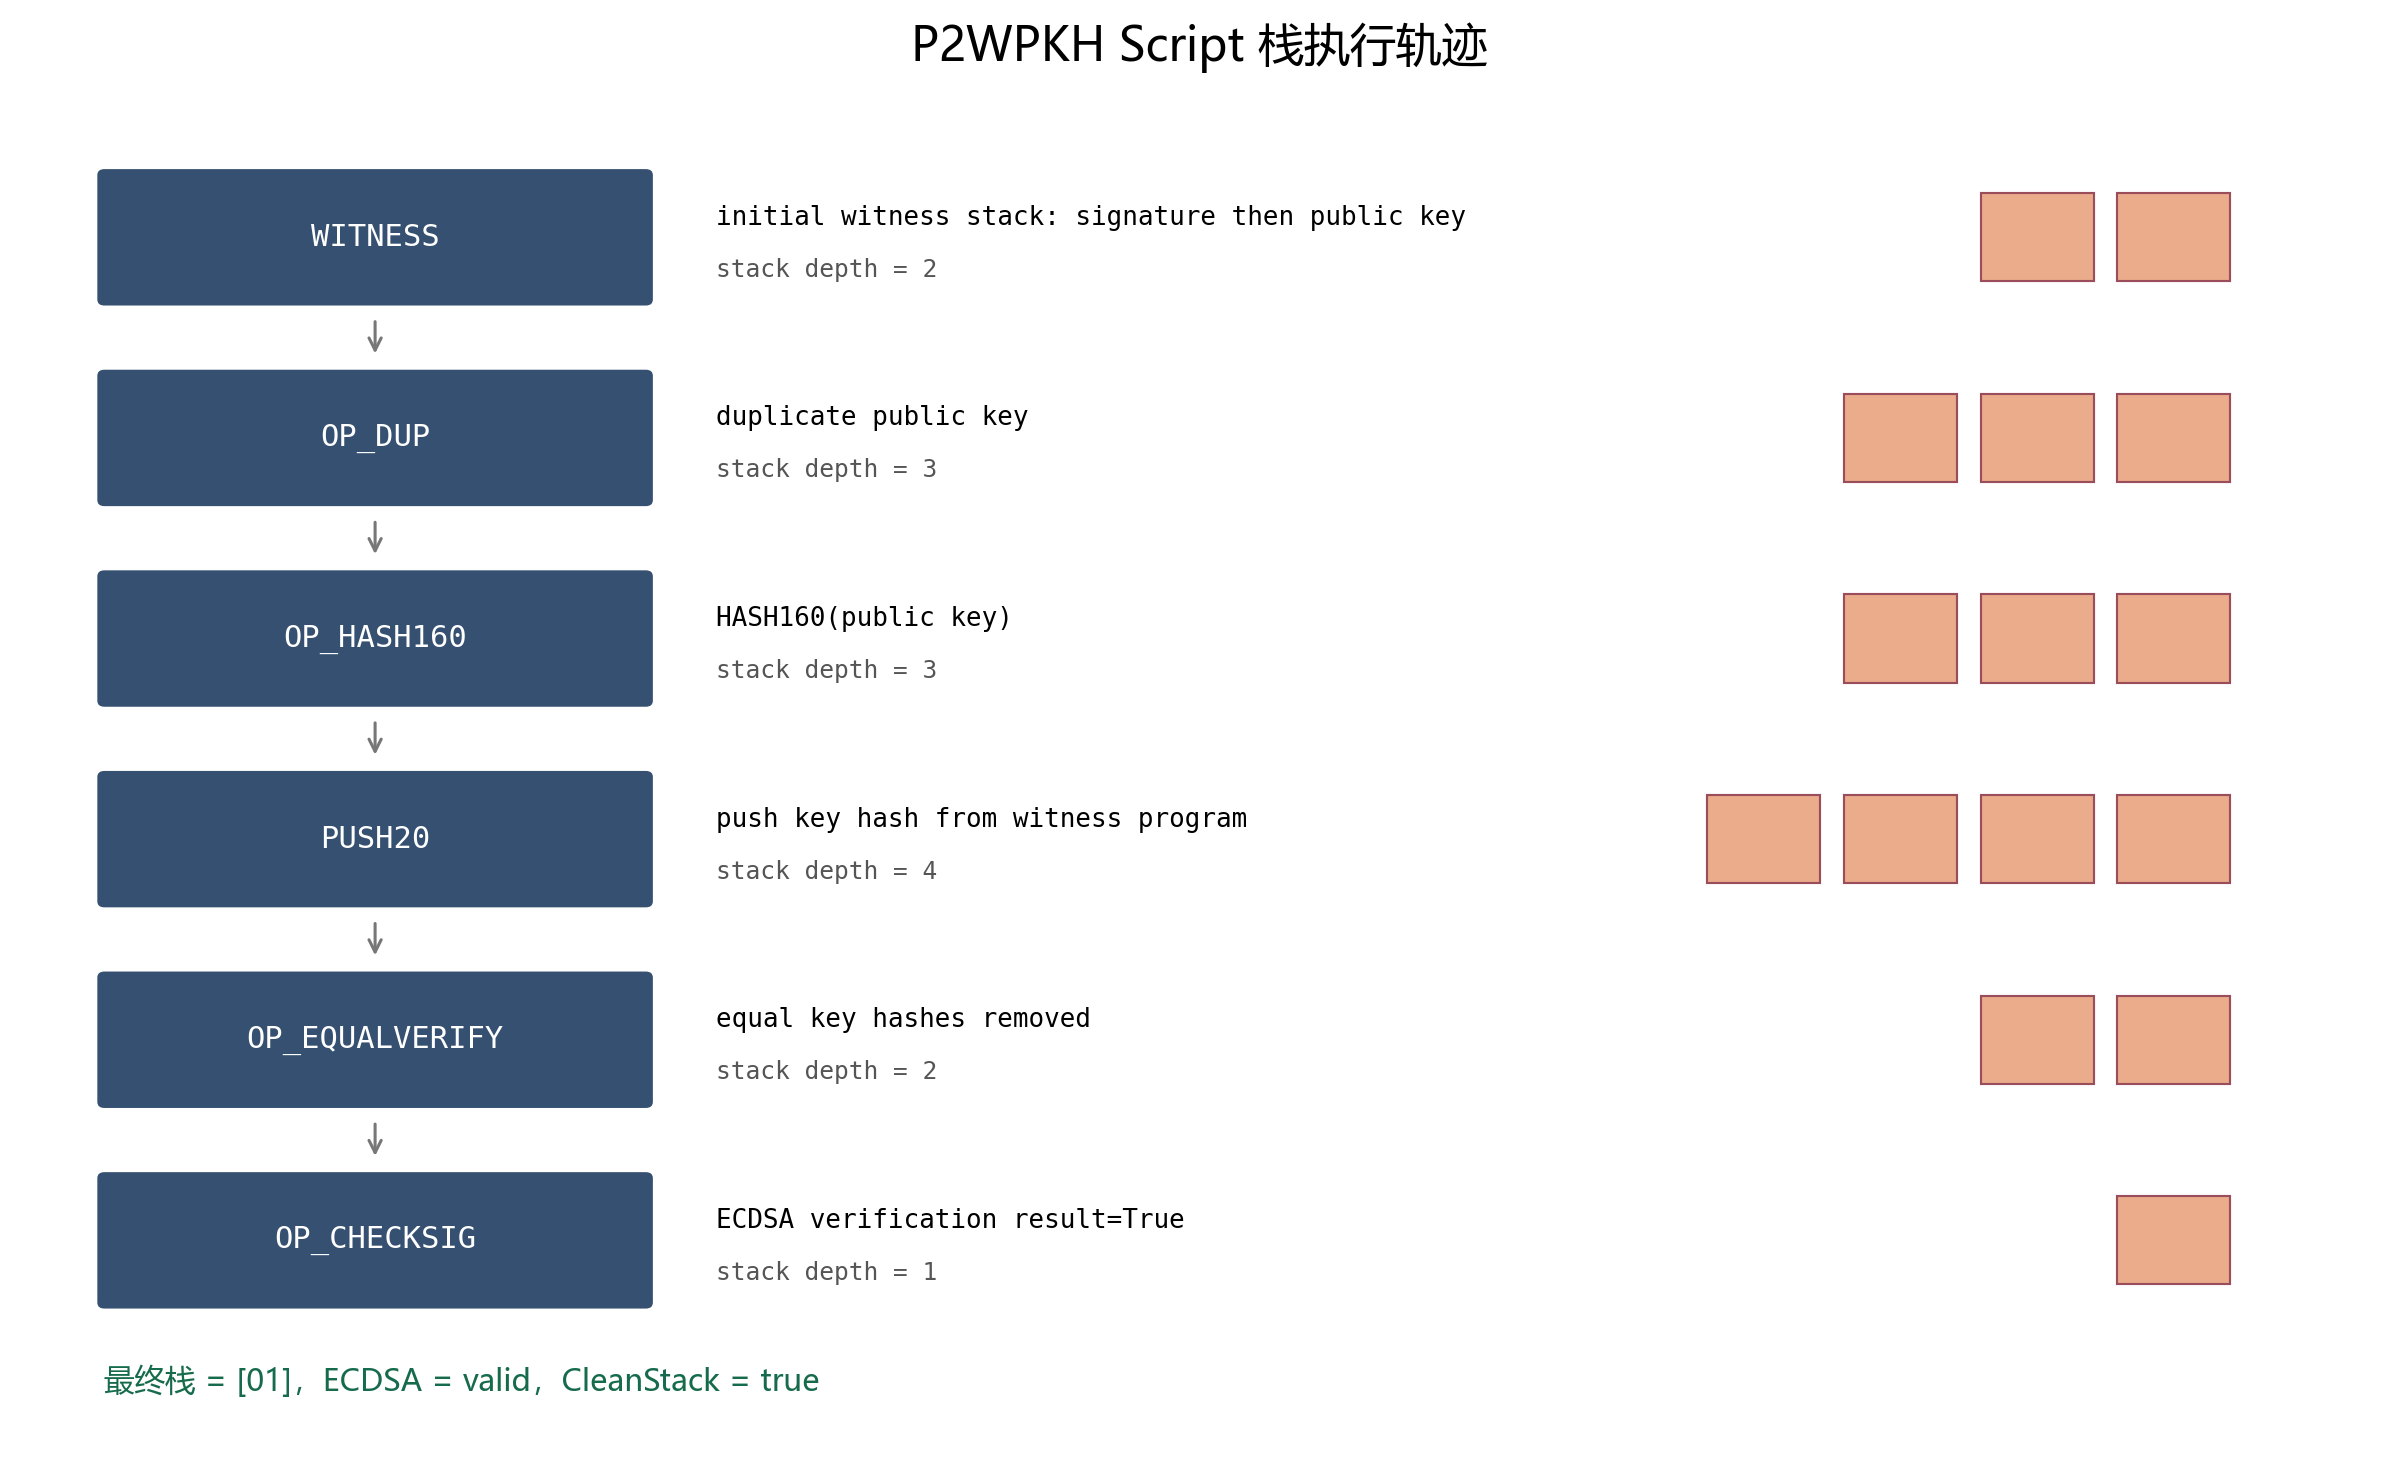
\includegraphics[width=0.94\textwidth]{../output/figures/script_stack_trace.png}
  \caption{P2WPKH Script 栈逐步执行结果}
  \label{fig:script-stack}
\end{figure}

\section{完整区块解析与 PoW 验证}

父交易随后在 Testnet4 高度 144878 获得确认，所在区块为
\texttt{\seqsplit{0000000000b9d2773b283332f6e1c36da7fdd7b11af12fa7f14866e0beb425ca}}。因此本节解析该真实包含父交易的完整区块；父交易位于交易索引 13（从 0 起，即区块内第 14 笔）。逐字节交易对象仍选用具有 BIP143/ECDSA 细节的子交易。最终采样时子交易尚未确认，故不虚构其与该区块之间的包含关系。

\begin{table}[H]
\centering
\caption{完整 Testnet4 区块独立重算结果}
\label{tab:block}
\begin{tabularx}{\textwidth}{p{0.27\textwidth} X}
\toprule
项目 & 值\\
\midrule
区块高度与大小 & 144878；4045 B，所有字节均被唯一字段覆盖\\
交易数 & 14，逐笔重序列化一致\\
version & 834363392\\
previous hash & \ttfamily\seqsplit{0000000000e9ed9d48999d673d817cf089298e111083a71670cc7c6b4faf856d}\\
头内 Merkle root & \ttfamily\seqsplit{5853640bbd50baf9df86ae513c514b856ba78e39933d2ea5fda3df2518edd102}\\
重算 Merkle root & 与头字段逐字节相等\\
timestamp & 1784541269（2026-07-20 09:54:29 UTC）\\
nBits & \texttt{0x1d00ffff}\\
target & \ttfamily\seqsplit{00000000ffff0000000000000000000000000000000000000000000000000000}\\
nonce & 1094189716\\
重算 block hash & \ttfamily\seqsplit{0000000000b9d2773b283332f6e1c36da7fdd7b11af12fa7f14866e0beb425ca}\\
PoW & $\operatorname{int}(hash)\le target$，通过\\
\bottomrule
\end{tabularx}
\end{table}

额外回归样本为默认 Signet 已确认交易
\texttt{\seqsplit{d083bf3e9d9eb467f9b1577b5d4b85174cce9d94f4c33f6d872d39e5d08c0689}}。其 235 B 交易、P2WPKH ECDSA、所在 74123 B 区块（41 笔交易）、Merkle 根和 PoW 均通过。这证明解析器并非只适配本实验构造的固定格式。

\section{测试、可复现性与结果讨论}

\subsection{自动化测试}

执行 \texttt{python -m unittest -v}，结果为：

\begin{lstlisting}[style=datastyle]
test_bech32_round_trip ................................ ok
test_compact_size_rejects_non_minimal_encoding ........ ok
test_complete_block_and_byte_accounting ............... ok
test_confirmed_transaction_and_script ................. ok
test_p2wsh_op_true_authorization ....................... ok
test_secp256k1_generator_and_ecdsa ..................... ok
----------------------------------------------------------------------
Ran 6 tests in 0.366s
OK
\end{lstlisting}

覆盖要点包括：标准 secp256k1 基点压缩公钥、签名消息篡改必须失败、low-S、DER 往返、Bech32 往返、非最短 CompactSize 必须拒绝、真实交易反序列化/重序列化、P2WPKH Script、P2WSH(OP\_TRUE)、完整区块 Merkle/PoW 与字节行数。

\subsection{复现实验命令}

在作业一根目录中运行：

\begin{lstlisting}[style=datastyle]
python -m unittest discover -s code -p "test_*.py" -v

python code/wallet_tool.py new --network testnet4 \
  --wallet data/testnet4_sender_wallet.json

python code/claim_op_true_utxos.py \
  --wallet data/testnet4_sender_wallet.json \
  --inputs 5 --output-value 1000 --broadcast

python code/wallet_tool.py send \
  --wallet data/testnet4_sender_wallet.json \
  --destination tb1qkts77kng6xv0rxldrjjfctk5jmf5nx3ltsndlw \
  --amount 400 --fee-rate 2 --allow-unconfirmed --broadcast \
  --output output/testnet4_signed_broadcast.json

python code/chain_analyzer.py --network testnet4 \
  --txid ad00f80a9c85264ebf3ca4299d61cca06efba0487223d4e6caa9d9e58e9ac105 \
  --block-hash 0000000000b9d2773b283332f6e1c36da7fdd7b11af12fa7f14866e0beb425ca \
  --output output/testnet4_signed_analysis

python code/visualize_results.py
\end{lstlisting}

\subsection{威胁模型与局限}

\begin{warningbox}[边界说明]
本实现是为了展示每个字节和每一步数学计算的课程代码，不是生产钱包。纯 Python 大整数点运算未承诺恒定时间；测试私钥只可用于无价值测试网络。程序验证本题涉及的 P2WPKH 与 P2WSH(OP\_TRUE)，并不宣称实现完整 Bitcoin Script 指令集或完整节点共识验证。REST API 只负责传输 raw bytes；真实性由本地 txid、block hash、Merkle 与 PoW 重算交叉检查。
\end{warningbox}

广播时父子交易均被 Testnet4 节点 mempool 接受；最终采样时父交易已经在高度 144878 确认，子交易仍未确认。mempool 接受证明交易已发送并通过节点策略验证，但不等同于最终确认；对子交易仍只陈述节点接受这一事实。报告同时保留 raw transaction、节点响应与本地重算结果，因此即使后续链上状态变化，实验数据仍可独立复核。

\section{结论}

本作业完成了原 Project 的四个核心动作：真实测试网发送、交易逐位/逐字节解析、完整区块解析以及 Script 逐步计算。父交易从 P2WSH witness program 出发验证公开 \texttt{OP\_TRUE} 授权并已在高度 144878 确认；子交易从 BIP143 原像出发完成 RFC6979/low-S ECDSA 签名并由节点接受。独立解析器对 223 B 子交易和包含父交易的 4045 B 区块做到无遗漏、无重叠映射，重算 txid、wtxid、Merkle 根、目标值和 PoW；Script 最终均为 CleanStack TRUE。默认 Signet 的已确认样本进一步验证实现的泛化性。结果文件与完整源代码共同构成可复现、可审计的交付。

\clearpage
\appendix
\section{完整逐字节结果文件索引}

\begin{longtable}{p{0.47\textwidth}p{0.43\textwidth}}
\toprule
相对路径 & 内容\\
\midrule
\endhead
\path{output/testnet4_signed_analysis/transaction_bits.txt} & 课程签名交易 223 个字节的 8 位展开\\
\path{output/testnet4_signed_analysis/transaction_fields.csv} & 字段起止偏移、wire hex、解释值\\
\path{output/testnet4_signed_analysis/script_audit.json} & BIP143 中间值、DER、ECDSA、Script 栈\\
\path{output/testnet4_signed_analysis/block_bits.txt} & 完整区块 4045 个字节的 8 位展开\\
\path{output/testnet4_signed_analysis/block_fields.csv} & 完整区块字段映射\\
\path{output/testnet4_signed_analysis/block_transaction_index.csv} & 14 笔交易的 txid/wtxid/size/weight/vsize\\
\path{output/testnet4_funding_analysis/script_audit.json} & 5 个 P2WSH(OP\_TRUE) 输入的执行轨迹\\
\path{output/sample_confirmed/} & 默认 Signet 已确认交易和 74123 B 区块回归结果\\
\bottomrule
\end{longtable}

\section{核心源代码}

以下代码均为本作业实际运行版本。

\subsection{bitcoin\_codec.py}
\lstinputlisting[style=pythonstyle]{../code/bitcoin_codec.py}

\subsection{wallet\_tool.py}
\lstinputlisting[style=pythonstyle]{../code/wallet_tool.py}

\subsection{claim\_op\_true\_utxos.py}
\lstinputlisting[style=pythonstyle]{../code/claim_op_true_utxos.py}

\subsection{chain\_analyzer.py}
\lstinputlisting[style=pythonstyle]{../code/chain_analyzer.py}

\subsection{visualize\_results.py}
\lstinputlisting[style=pythonstyle]{../code/visualize_results.py}

\subsection{test\_bitcoin\_codec.py}
\lstinputlisting[style=pythonstyle]{../code/test_bitcoin_codec.py}

\clearpage
\begin{thebibliography}{99}

\bibitem{bip94}
Fabian Jahr. \textit{BIP 94: Testnet 4}. Bitcoin BIPs, 2024.\
\url{https://github.com/bitcoin/bips/blob/master/bip-0094.mediawiki}. 访问日期：2026-07-20.

\bibitem{bip141}
Eric Lombrozo, Johnson Lau, Pieter Wuille. \textit{BIP 141: Segregated Witness (Consensus layer)}. Bitcoin BIPs, 2015.\
\url{https://github.com/bitcoin/bips/blob/master/bip-0141.mediawiki}. 访问日期：2026-07-20.

\bibitem{bip143}
Johnson Lau, Pieter Wuille. \textit{BIP 143: Transaction Signature Verification for Version 0 Witness Program}. Bitcoin BIPs, 2016.\
\url{https://github.com/bitcoin/bips/blob/master/bip-0143.mediawiki}. 访问日期：2026-07-20.

\bibitem{bip173}
Pieter Wuille, Greg Maxwell. \textit{BIP 173: Base32 address format for native v0-16 witness outputs}. Bitcoin BIPs, 2017.\
\url{https://github.com/bitcoin/bips/blob/master/bip-0173.mediawiki}. 访问日期：2026-07-20.

\bibitem{bip325}
Karl-Johan Alm, Anthony Towns. \textit{BIP 325: Signet}. Bitcoin BIPs, 2019.\
\url{https://github.com/bitcoin/bips/blob/master/bip-0325.mediawiki}. 访问日期：2026-07-20.

\bibitem{nakamoto}
Satoshi Nakamoto. \textit{Bitcoin: A Peer-to-Peer Electronic Cash System}. 2008.\
\url{https://bitcoin.org/bitcoin.pdf}. 访问日期：2026-07-20.

\bibitem{devref}
Bitcoin.org. \textit{Bitcoin Developer Reference: Transactions and Block Chain}.\
\url{https://developer.bitcoin.org/reference/transactions.html};
\url{https://developer.bitcoin.org/reference/block_chain.html}. 访问日期：2026-07-20.

\bibitem{mempoolapi}
The Mempool Open Source Project. \textit{mempool REST API Documentation}.\
\url{https://github.com/mempool/mempool/blob/master/docs/api/rest.md}. 访问日期：2026-07-20.

\bibitem{rfc6979}
T. Pornin. \textit{RFC 6979: Deterministic Usage of the Digital Signature Algorithm (DSA) and Elliptic Curve Digital Signature Algorithm (ECDSA)}. IETF, 2013.\
\url{https://www.rfc-editor.org/rfc/rfc6979}. 访问日期：2026-07-20.

\end{thebibliography}

\end{document}
